\documentclass[11pt]{report}
\usepackage{graphics}
\usepackage{anysize}
\marginsize{3cm}{3cm}{3cm}{2cm}
\def\thesection{}%\arabic{section}} 
\pagenumbering{Roman}

\begin{document}
\newpage
\section{Appendix E: Development Statistics}
{
\begin{figure}[h]
\centering
\scalebox{0.6} {
	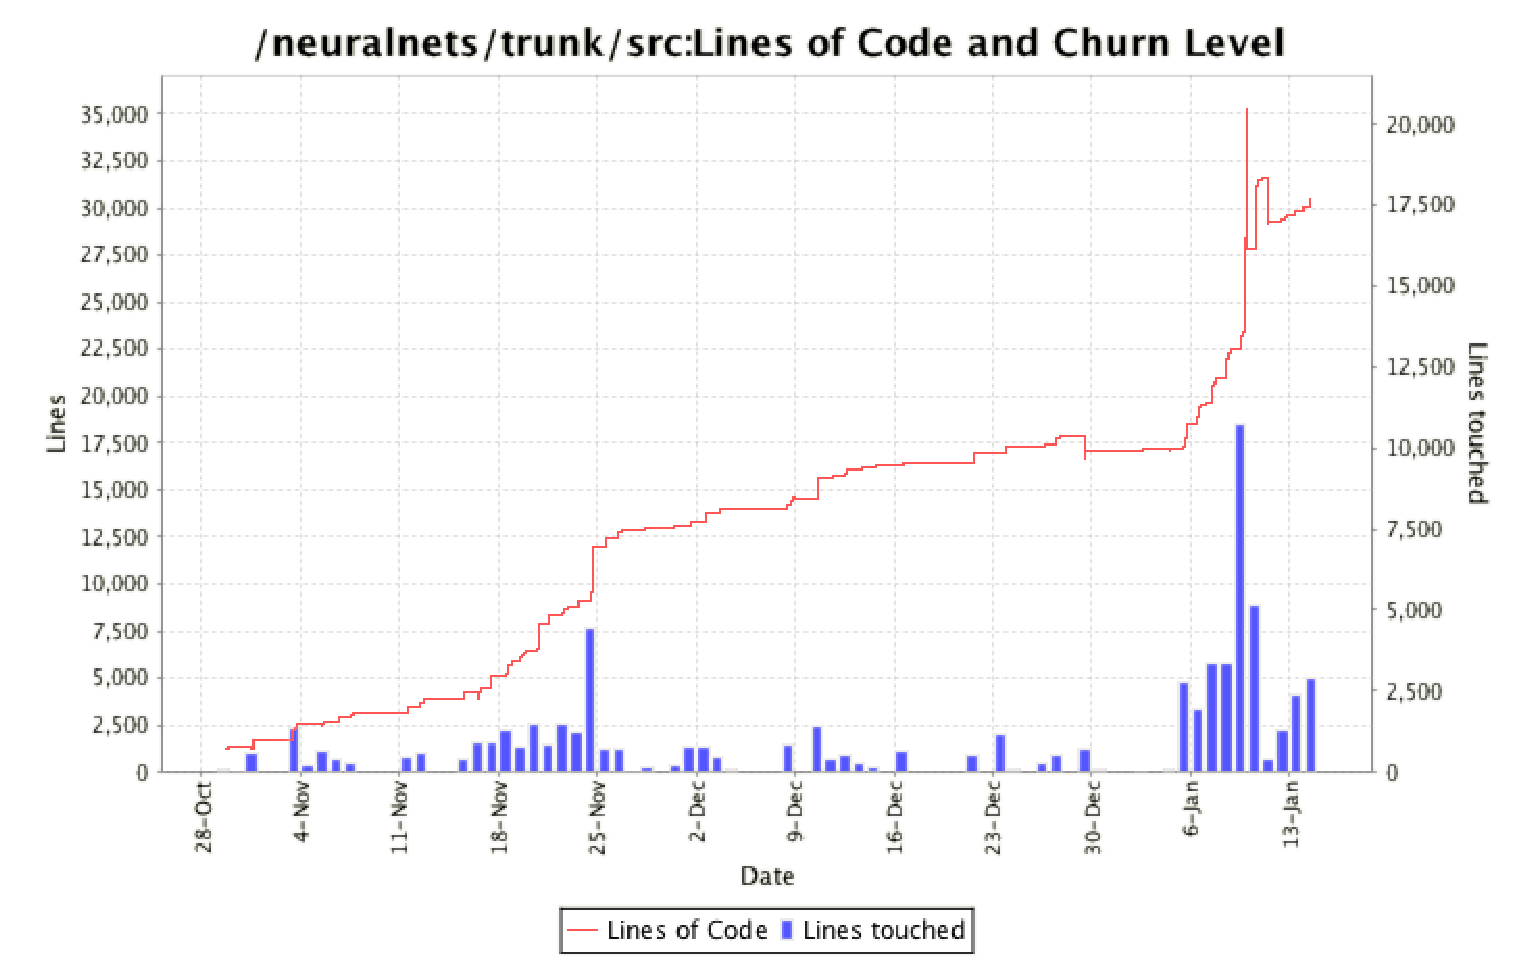
\includegraphics{locandchurn}
}
\caption{LOC and Churn Diagram: Note the period of architectural refactoring etowards the end of the project, increasing churn and line count significantly.}
\label{fig:gui}
\end{figure}

\begin{figure}[h]
\centering
\scalebox{0.6} {
	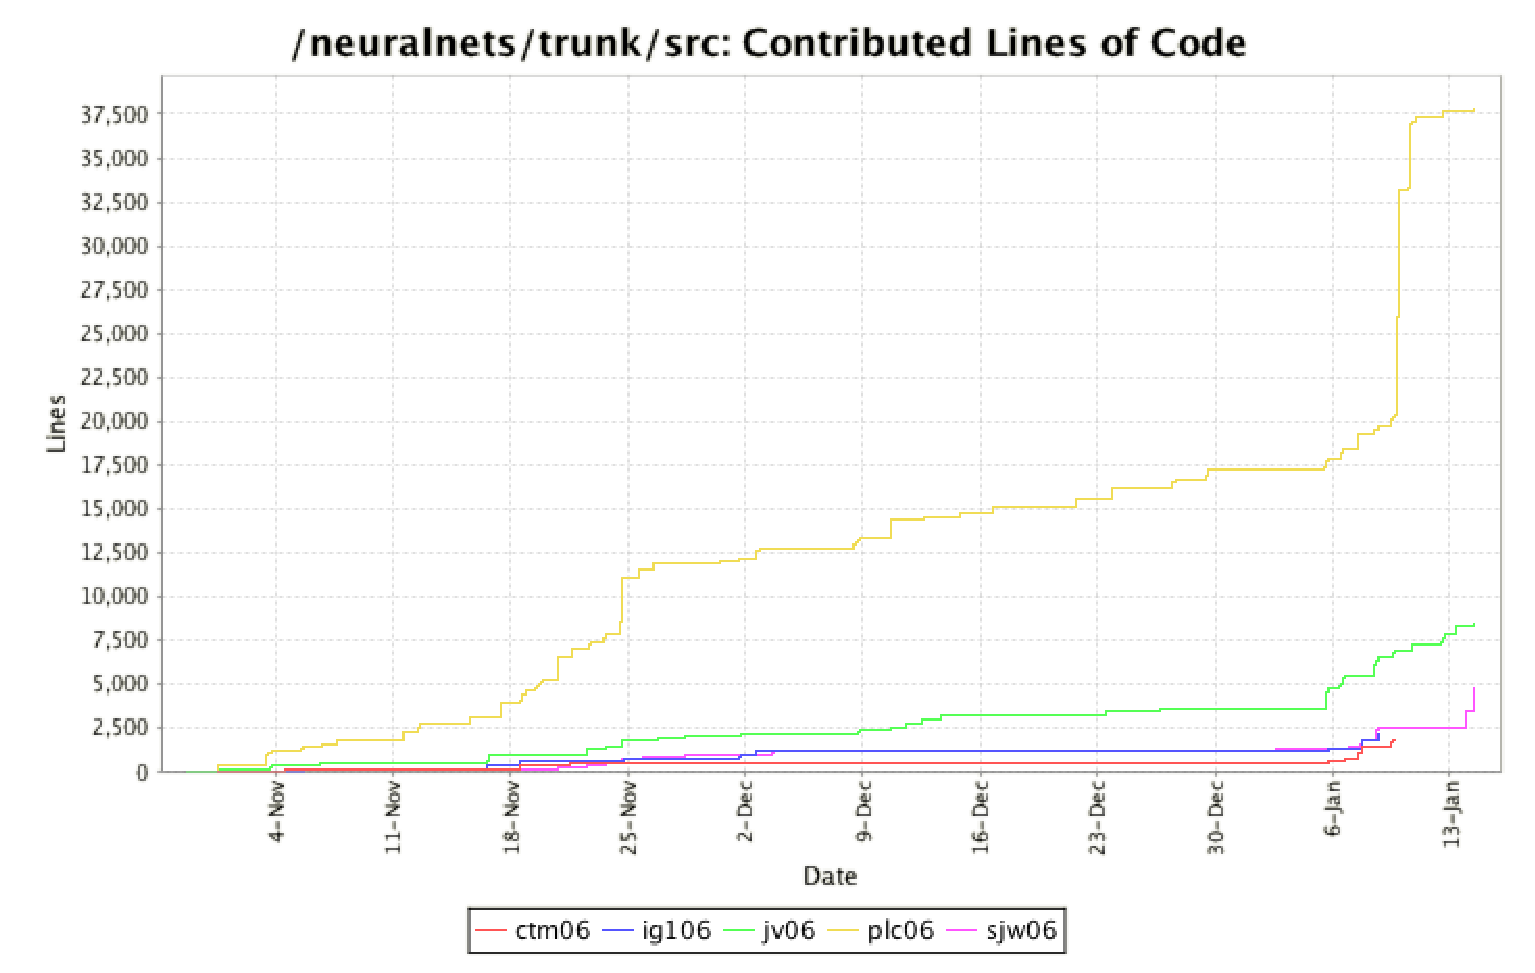
\includegraphics{locperauthor}
}
\caption{LOC Breakdown per Author: Provides interesting view of pair programming practices; apparent reduction in LOC productivity per developer may well be offset by quality of code produced.}
\label{fig:util}
\end{figure}

\begin{figure}[h]
\centering
\scalebox{0.6} {
	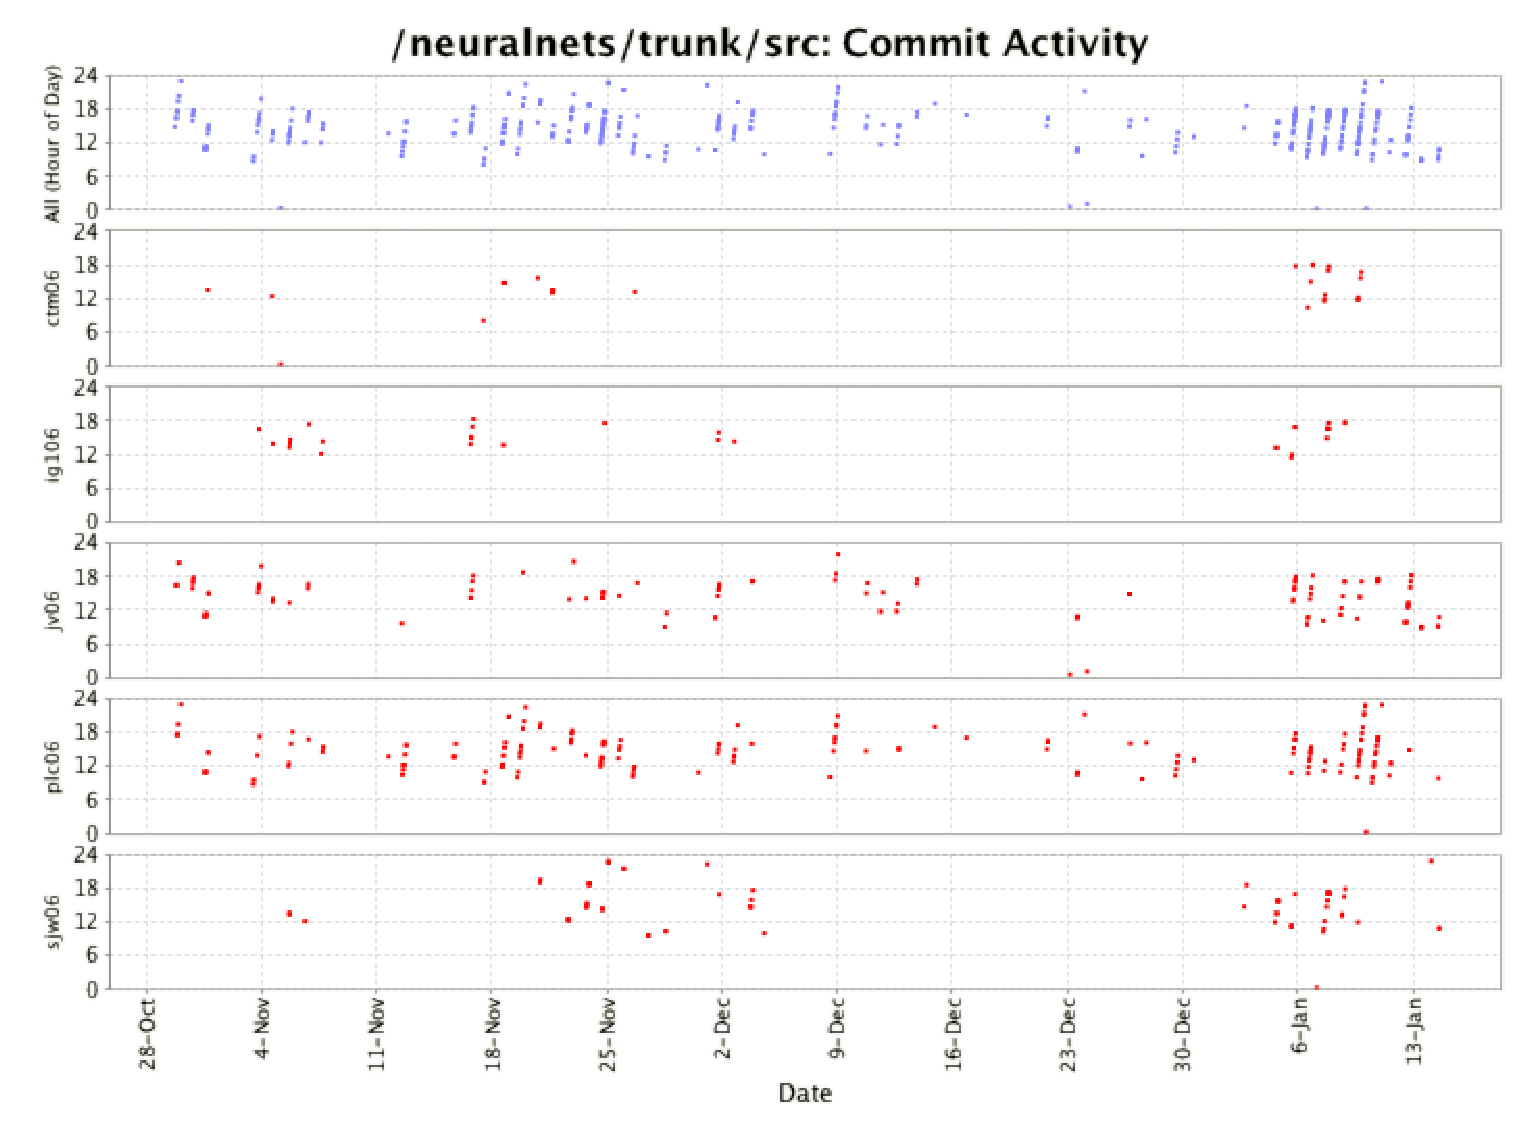
\includegraphics{commitscatterauthors}
}
\caption{Scatter plot of commit activity by date and time.}
\label{fig:ast}
\end{figure}

\begin{figure}[h]
\centering
\scalebox{0.6} {
	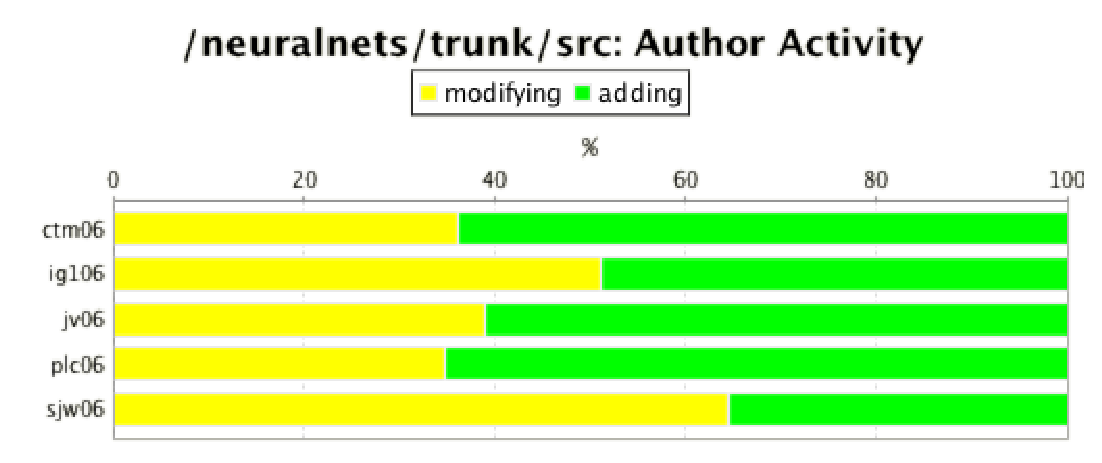
\includegraphics{activity}
}
\caption{Overall creation and churn activity. Lower churn for pair programmers is evident here, supplying evidence for the improved quality of their code.}
\label{fig:persistence}
\end{figure}
}
\end{document}
